\subsection{Application Measurements}\label{sec:application:cloud_file_synchronisation:application_measurements}
The model presented in \refsec{model} requires several input parameters which are obtained from measurements and described in this section.
In \refsec{sec:application:cloud_file_synchronisation:application_measurements:bandwidth_preparation_times} we first give an overview over the measurement setup implemented in the distributed testbed PlanetLab~\cite{Chun2003}.
Then we present measurement results as well as fitted distributions for both up and download bandwidth as well as for the time used by the cloud service to prepare data prior to the download.
Finally, in \refsec{sec:application:cloud_file_synchronisation:application_measurements:image_file_sizes} we derive a image file size distribution by analysing a large set of digital photos.

\subsubsection*{Bandwidth and Preparation Times}\label{sec:application:cloud_file_synchronisation:application_measurements:bandwidth_preparation_times}
We obtain a PlanetLab slice containing all available nodes in February 2014 and discard every node not responding to \texttt{ping} or \texttt{ssh} within a \SI{20}{\second} interval.
On the remaining \(87\) nodes we install our measurement setup.
This includes two instances of the \dropbox client on each host, linking them to a specially created \dropbox account and two different directories.
Furthermore, we disable the \emph{LAN-Synchronization} feature for both clients.
After ensuring that both shared directories are empty, we create a file with randomly generated content of \SI{10}{\mega\bit} size, unique per node.
Files are unique in order to compensate for caching algorithms by \dropbox, as the client calculates a checksum of the file prior to uploading and only uploads the file if no duplicate file is already stored in the account, in order to conserve bandwidth.
Further, the randomly generated content ensures that no significant compression results can be achieved before uploading, resulting in comparable results for the time required to upload the files.
After the file is created, we start \texttt{tcpdump} and \emph{symlink} the file to the first directory shared via \dropbox while taking note of the \emph{initial timestamp} of the symlink.
As the complete file has finished downloading and appears in the second \dropbox directory, we note the current \emph{final timestamp} and stop \texttt{tcpdump}.
Finally, we retrieve the traffic dump and the recorded timestamps and reset the measurement setup.

\begin{figure}
  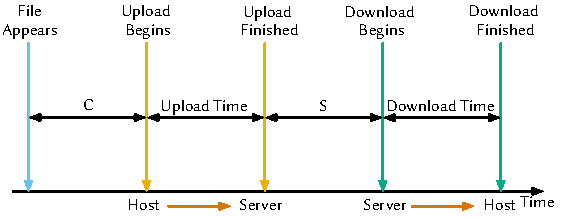
\includegraphics{application/cloud_file_synchronization/application_measurements/figures/measurement_setup}
  \caption{Measurement Setup}
  \label{fig:application:cloud_file_synchronisation:application_measurements:bandwidth_preparation_times:measurement_setup}
\end{figure}

This process is repeated \(8\) times for all available PlanetLab nodes.
Based on the two recorded timestamps as well as the traffic dump, we calculate the required values for the model as shown in \reffig{fig:application:cloud_file_synchronisation:application_measurements:bandwidth_preparation_times:measurement_setup}.
The time between the \emph{inital timestamp} and the first packet sent to the \emph{Amazon S3} storage server is considered the client preparation time \clientpreparationtime.

\subsubsection*{Image File Sizes}\label{sec:application:cloud_file_synchronisation:application_measurements:image_file_sizes}

